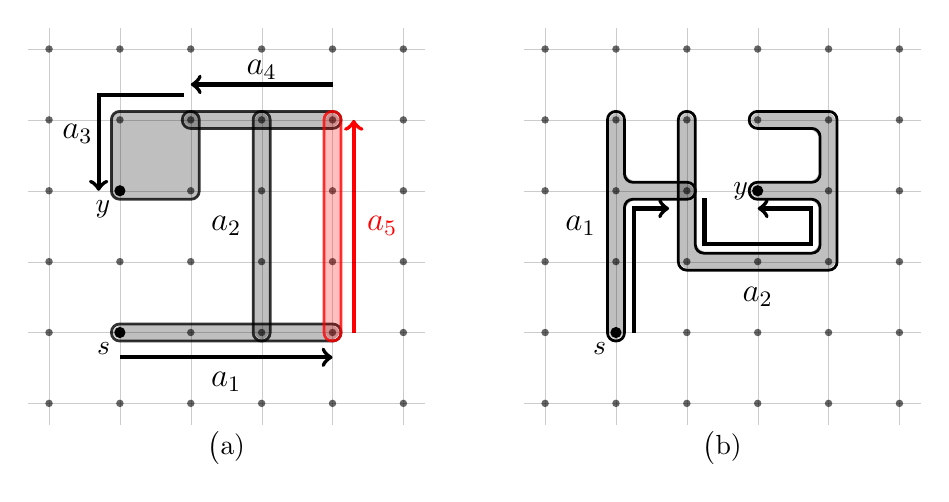
\begin{tikzpicture}[scale=0.9]
\definecolor{b1}{RGB}{0, 0, 0}
\definecolor{b2}{RGB}{4, 75, 145}
\definecolor{b3}{RGB}{76, 68, 194}
\definecolor{b4}{RGB}{50, 140, 190}
\draw[->, line width=1.5] (0, -0.35) -- (3, -0.35);
%\draw[->, dashed, red, line width=1.5] (3.35, 3) -- (3.35, 0);
\draw[<-, red, line width=1.5] (3.3, 3) -- (3.3, 0);
\draw[->, line width=1.5] (3, 3.5000000000000003) -- (1, 3.5000000000000003);
%\draw[<-, dashed, line width=1.5] (3, 3.45) -- (1.1, 3.45);
%\draw[->, dashed, line width=1.5] (1.35, 2) -- (1.35, 2.85);
\draw[->, line width=1.5] (0.9, 3.35) -- (-0.3, 3.35) -- (-0.3, 2);
\def\wi{0.08}
\def\op{0.2}
\def\pts{2.0pt}

\foreach \y in {-1, ...,4} {
\draw[black, line width=\wi, opacity=\op] (-1.3, \y) -- (4.3, \y);
\draw[black, line width=\wi, opacity=\op] (5.7, \y) -- (11.3, \y);
%\draw[black, line width=\wi, opacity=\op] (-46.3, \y) -- (-28.7, \y);
}
\foreach \x in {-1, 0, 1, 2, 3, 4, 6, 7, 8, 9, 10, 11} {
\draw[black, line width=\wi, opacity=\op] (\x, -1.3) -- (\x, 4.3);
%\draw[black, line width=\wi, opacity=\op] (\x, 5.7) -- (\x, 11.3);
%\draw[black, line width=\wi, opacity=\op] (-46.3, \y) -- (-28.7, \y);
}

% \foreach \y in {0,...,23} {
% \draw[black, line width=\wi, opacity=\op] (-25.3, \y) -- (3.3, \y);
% \draw[black, line width=\wi, opacity=\op] (-46.3, \y) -- (-28.7, \y);
% }

\foreach \x in {-1,...,4} {
\foreach \y in {-1,...,4} {
\fill[black, opacity=0.6] (\x, \y) circle (1.5pt);
}
}
\foreach \x in {6,...,11} {
\foreach \y in {-1,...,4} {
\fill[black, opacity=0.6] (\x, \y) circle (1.5pt);
}
}
\draw[b1, line width=1pt, opacity=0.8, rounded corners=3pt] (-0.12, -0.12) rectangle (3.12, 0.12);
\fill[b1, opacity=0.25, rounded corners=5pt] (-0.12, -0.12) rectangle (3.12, 0.12);

\draw[b1, line width=1pt, opacity=0.8, rounded corners=3pt] (1.88, -0.12) rectangle (2.12, 3.12);
\fill[b1, opacity=0.25, rounded corners=5pt] (1.88, -0.12) rectangle (2.12, 3.12);
\draw[b1, line width=1pt, opacity=0.8, rounded corners=3pt] (0.88, 2.88) rectangle (3.12, 3.12);
\fill[b1, opacity=0.25, rounded corners=5pt] (0.88, 2.88) rectangle (3.12, 3.12);
\draw[red, line width=1pt, opacity=0.8, rounded corners=3pt] (2.88, -0.12) rectangle (3.12, 3.12);
\fill[red, opacity=0.25, rounded corners=5pt] (2.88, -0.12) rectangle (3.12, 3.12);
\draw[b1, line width=1pt, opacity=0.8, rounded corners=3pt] (-0.12, 1.88) rectangle (1.12, 3.12);
\fill[b1, opacity=0.25, rounded corners=3pt] (-0.12, 1.88) rectangle (1.12, 3.12);
\draw[black, line width=1pt, rounded corners=3pt](7.88, 3.12) -- (7.88, 0.88) -- (10.120000000000001, 0.88) -- (10.120000000000001, 3.12) -- (8.88, 3.12) -- (8.88, 2.88) -- (9.879999999999999, 2.88) -- (9.879999999999999, 2.12) -- (8.88, 2.12) -- (8.88, 1.88) -- (9.879999999999999, 1.88) -- (9.879999999999999, 1.12) -- (8.12, 1.12) -- (8.12, 3.12) -- cycle;
\fill[black, opacity=0.25, rounded corners=5pt](7.88, 3.12) -- (7.88, 0.88) -- (10.120000000000001, 0.88) -- (10.120000000000001, 3.12) -- (8.88, 3.12) -- (8.88, 2.88) -- (9.879999999999999, 2.88) -- (9.879999999999999, 2.12) -- (8.88, 2.12) -- (8.88, 1.88) -- (9.879999999999999, 1.88) -- (9.879999999999999, 1.12) -- (8.12, 1.12) -- (8.12, 3.12) -- cycle;
\draw[black, line width=1pt, rounded corners=3pt](6.88, -0.12) -- (6.88, 3.12) -- (7.12, 3.12) -- (7.12, 2.12) -- (8.120000000000001, 2.12) -- (8.120000000000001, 1.88) -- (7.12, 1.88) -- (7.12, -0.12) -- cycle;
\fill[black, opacity=0.25, rounded corners=5pt](6.88, -0.12) -- (6.88, 3.12) -- (7.12, 3.12) -- (7.12, 2.12) -- (8.120000000000001, 2.12) -- (8.120000000000001, 1.88) -- (7.12, 1.88) -- (7.12, -0.12) -- cycle;
%\draw[->, dashed, line width=1.5] (6.75, 1) -- (6.75, 0);
\draw[->, line width=1.5] (7.25, 0) -- (7.25, 1.75) -- (7.75, 1.75);
\draw[->, line width=1.5] (8.25, 1.9) -- (8.25, 1.25) -- (9.75, 1.25) -- (9.75, 1.75) -- (9, 1.75);
%\draw[->, dashed, line width=1.5] (8.25, 3) -- (8.25, 2.1);
\filldraw (7, 0) circle (2pt);
\node[below left] at (7, 0) {$s$};
\filldraw (0, 2) circle (2pt);
\node[below left] at (0, 2) {$y$};
\filldraw (9, 2) circle (2pt);
\node[left] at (9, 2) {$y$};
\filldraw (0, 0) circle (2pt);
\node[below left] at (0, 0) {$s$};
% \filldraw[red] (3, 3) circle (2pt);
% \node[above right] at (3, 3) {\textcolor{red}{$p_5$}};
% \filldraw (2, 3) circle (2pt);
\node[] at (9, 0.5) {\large $a_2$};
\node[] at (1.5, 1.5) {\large $a_2$};
\node[] at (1.5, -0.7) {\large $a_1$};
\node[] at (6.5, 1.5) {\large $a_1$};
\node[red] at (3.7, 1.5) {\large $a_5$};
\node[] at (-0.6, 2.8) {\large $a_3$};
\node[] at (2, 3.7) {\large $a_4$};
% \filldraw (1, 2) circle (2pt);
% \node[below right] at (1, 2) {$p_3$};
% \filldraw (1, 3) circle (2pt);
% \node[above right] at (1, 3) {$p_4$};
% \filldraw (0, 3) circle (2pt);
% \node[above left] at (0, 3) {$y$};
% \filldraw (7, 1) circle (2pt);
% \node[above left] at (7, 1) {$p_1$};
% \filldraw (8, 3) circle (2pt);
%\node[above] at (8, 3) {$p_2$};
\node[above] at (1.5, -2) {\big (a)};
\node[above] at (8.5, -2) {\big (b)};
\end{tikzpicture}
%[Finished in 0.2s]